\documentclass[0-suturing.tex]{subfiles}
\begin{document}

%==START SECTION==============================
\section{Introduction}
\label{sec:intro}
%============================================
Robot-assisted surgical systems in Minimally Invasive Surgery (RMIS)
have facilitated pairing of human surgical expertise with the precision and repeatability of robots. Intuitive Surgical's da Vinci Robotic Surgical Assistant, a type of RSA, facilitated over $570,000$ procedures worldwide in $2014$ with $3000$ systems~\cite{AnnualReport2014}.
In spite of the growing prevalence of the robot-assisted minimally invasive surgery (RMIS), manual control under tele-operation limits 
the benefits of using a robotic system, particularly in frequently repeated sub-tasks such as suturing, knot-tying, resections and so on. 

% Usage of robotic minimally invasive surgical systems for general surgical procedures is growing rapidly. But current systems are under direct tele-operated control. Introducing autonomy has many benefits including:
% Reducing surgeon fatigue
% Enabling remote tele-surgery
% Enabling superhuman performance

% Robotic surgical systems used in Minimally Invasxive Surgery (MIS) present an opportunity to pair human surgical expertise with the precision and repeatability of robots. There are numerous reasons why the automation of surgical tasks can be useful.
% First the automation of tedious and repetitive can provide with surgeons with breaks and reduced fatigue during lengthy procedures.
% Furthermore robotic automation can allow the robot to perform tasks with increased dexterity and precision at superhuman speeds.
% Current tele-operation systems cannot be controlled remotely over long distances due to transmission delays. Surgical automation can enable remote surgery by providing surgeons with a supervisory role and high level commands to direct the robot to desired suture locations.

We have explored the automation of continuous/running suturing task in this paper. It is a suturing technique that involves multiple sequential sutures without knot tying between consecutive needle insertions. Running sutures are useful for long wounds in which wound tension has been minimized with properly placed deep sutures and in which approximation of the wound edges is good. It helps in a gradual approximation of tissue edges and is less time-consuming when compared to interrupted sutures. The continuous suturing technique has been widely used in surgical practice\tocite in complex procedures such as  anastomosis\tocite. 

% Continuous running suturing is a suturing technique that does not require knot tying in between each stitch, allowing for faster task completion.
% We are interested in automating continuous surgical suturing because:
% It is a frequently used and important task in surgery 
% (support with citation, Cavusoglu et al icra15 and t-ro15 paper)

Although, continuous suturing is so frequently used, it remains a tedious and time consuming task. Automating this suturing technique may reduce both the time and difficulty associated with suturing. Research in suturing poses questions in (a) interaction with deformable tissue, (b) multilateral manipulation of needle and suture, and (c) hierarchical models for multi-step task planning. We note the research focus on this topic has explored at a subset of these questions~\todo{Cavusoglu et al icra15 and t-ro15 paper}. However, a combination of these contributes to the complexity of fully autonomous operation.
% Autonomous robotic manipulation and control of the suture needle and thread would allow the robot to complete the suture while relying on minimal guidance from the surgeon. 

\begin{figure}[!t]
\centering
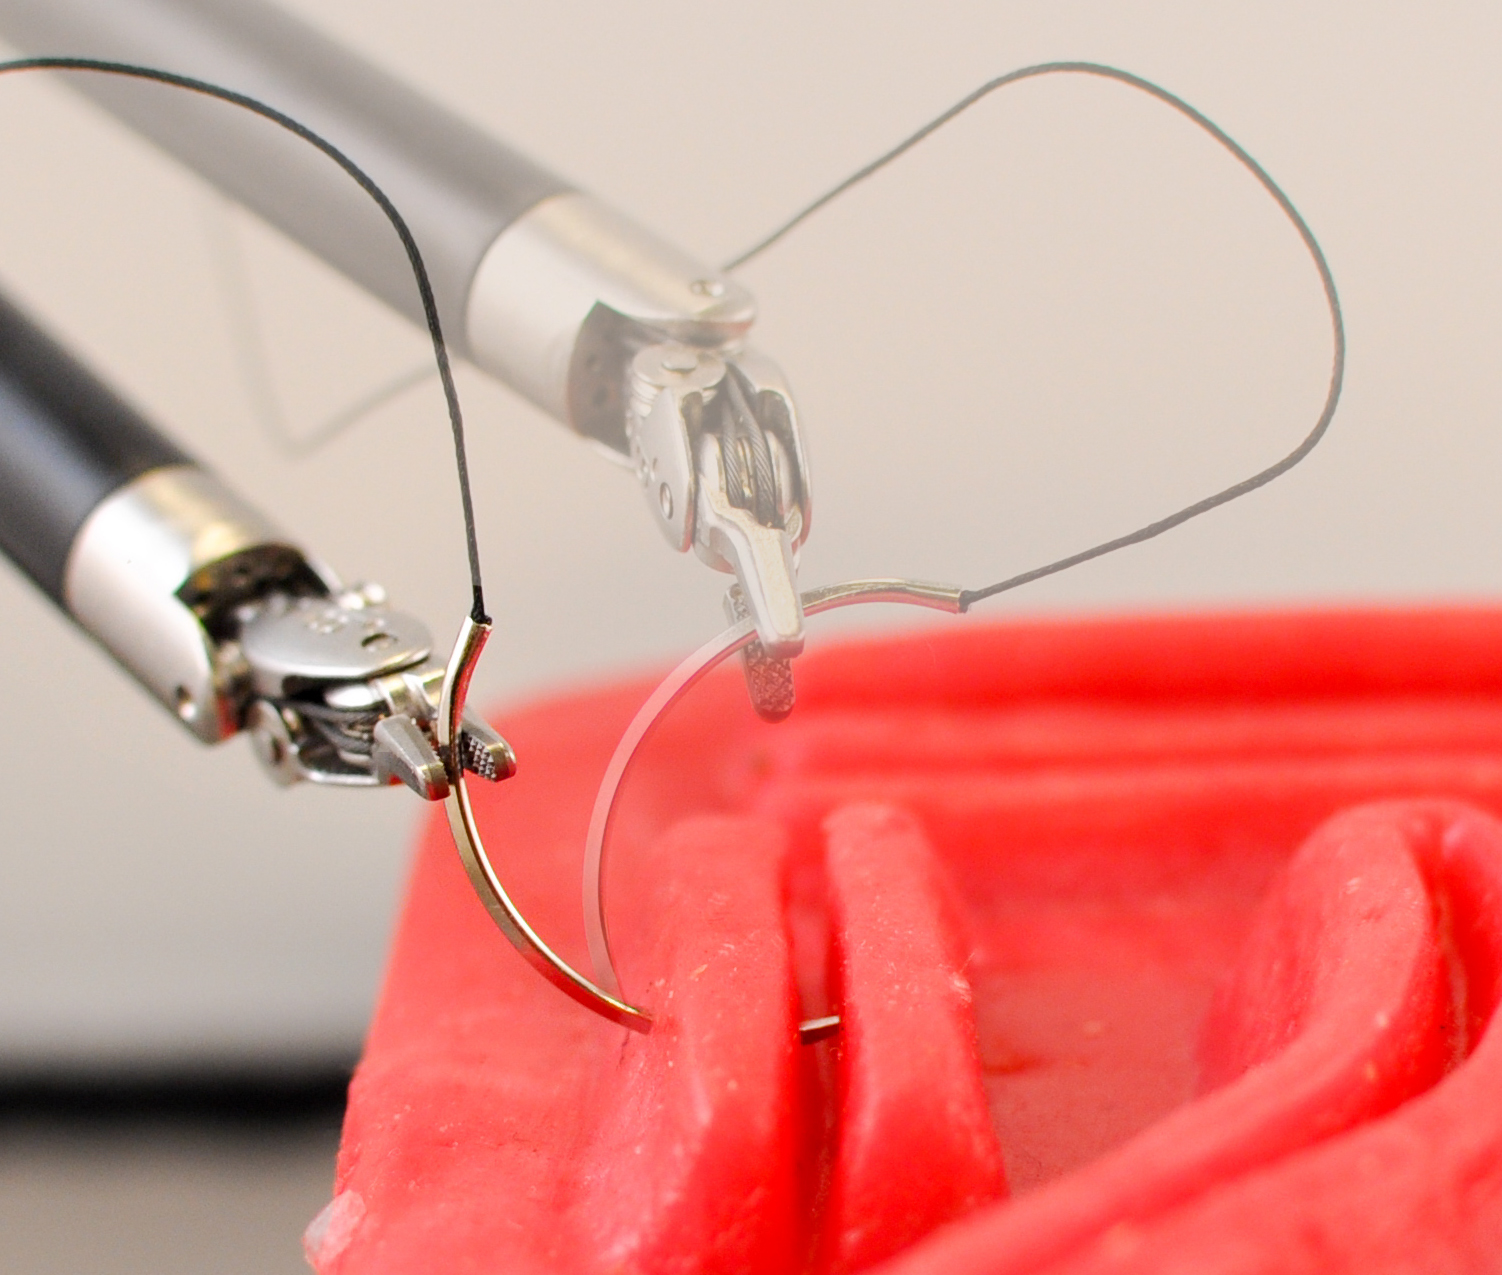
\includegraphics[width=0.9\linewidth]{figures/NeedleInsertionCombo}
% \vspace{-5pt}
\caption{\todo{placeholder} The figure illustrates the steps in autonomous suturing needle insertion step as a time lapse overlay labelled 1, 2, 3, 4. This figure has the complex suturing setup with long running flexible vertical targets. The robot performs [n??] throws of suture in [t??] sec.}
\label{fig:intro}
\vspace{-10pt}
\end{figure}

This paper presents preliminary results towards the automation of the continuous suturing task. We propose a framework of software and hardware that enables robust automation of the continuous suturing task. 
This paper builds upon prior art in optimization based planning with uncertainty\cite{patil2014gaussian},\todo{others}, segmentation of task demonstrations\cite{krishnan2015tsc, lea2015improved}, and building \& tuning finite state machines\cite{Murali2015Learning}. We present a robust segmentation of the single throw suturing task, and build upon the state machine to enable multi-throw running suturing. Each suturing throw is formulated as a curvature constrained trajectory optimization over the pose of the needle leveraging a belief space planning framework. Furthermore, real time needle tracking along with closed loop needle hand-off is demonstrated on the Intuitive Surgical dVRK \cite{Kazanzides2014}. We also present a novel low-cost passive gripper jaw mount for needle alignment. The device allows automatic needle re-positioning, reducing the effort in multilateral needle manipulation to achieve near optimal orientation for needle insertion.

Our system uses an elegant interface allowing the surgeon to trace the wound using the tool tip. Moreover, given one a suture width and a wound depth, the system calculated the required number of suture throws with corresponding entry and exit points. Our system can also be generalized to take a mesh of the incision as a input to the suturing task. The full procedure is performed with closed loop needle tracking and the needle path planner accounts for uncertainty in the needle pose estimation.

\vspace{5pt}
\noindent \textbf{Contributions}:
\begin{enumerate}[noitemsep, leftmargin=*]
\item Robust closed loop Finite State Machine for Continuous Suturing with needle tracking and multilateral needle hand-off. Belief Space Planning based Needle Trajectory Generation and needle size selection.
\item Gripper Jaw mount for automatic needle orientation during grasping for minimizing uncertainty during multilateral manipulation.
\item 4-Throw Continuous Suturing Task as recommended by FRSR~\cite{stegemann2013fundamental}\todo{check paper}. Evaluation on Objective Structured Assessment of Technical Skills (OSATS)~\cite{schreuder2012training} and comparison with manual demonstrations of varying skill levels (expert, intermediates and novices) from the JIGSAWS dataset~\cite{gao2014jhu}. Higher complexity suturing task with vertical walls, evaluation of robustness and time to completion.
\end{enumerate}


\begin{figure*}[!t]
\centering
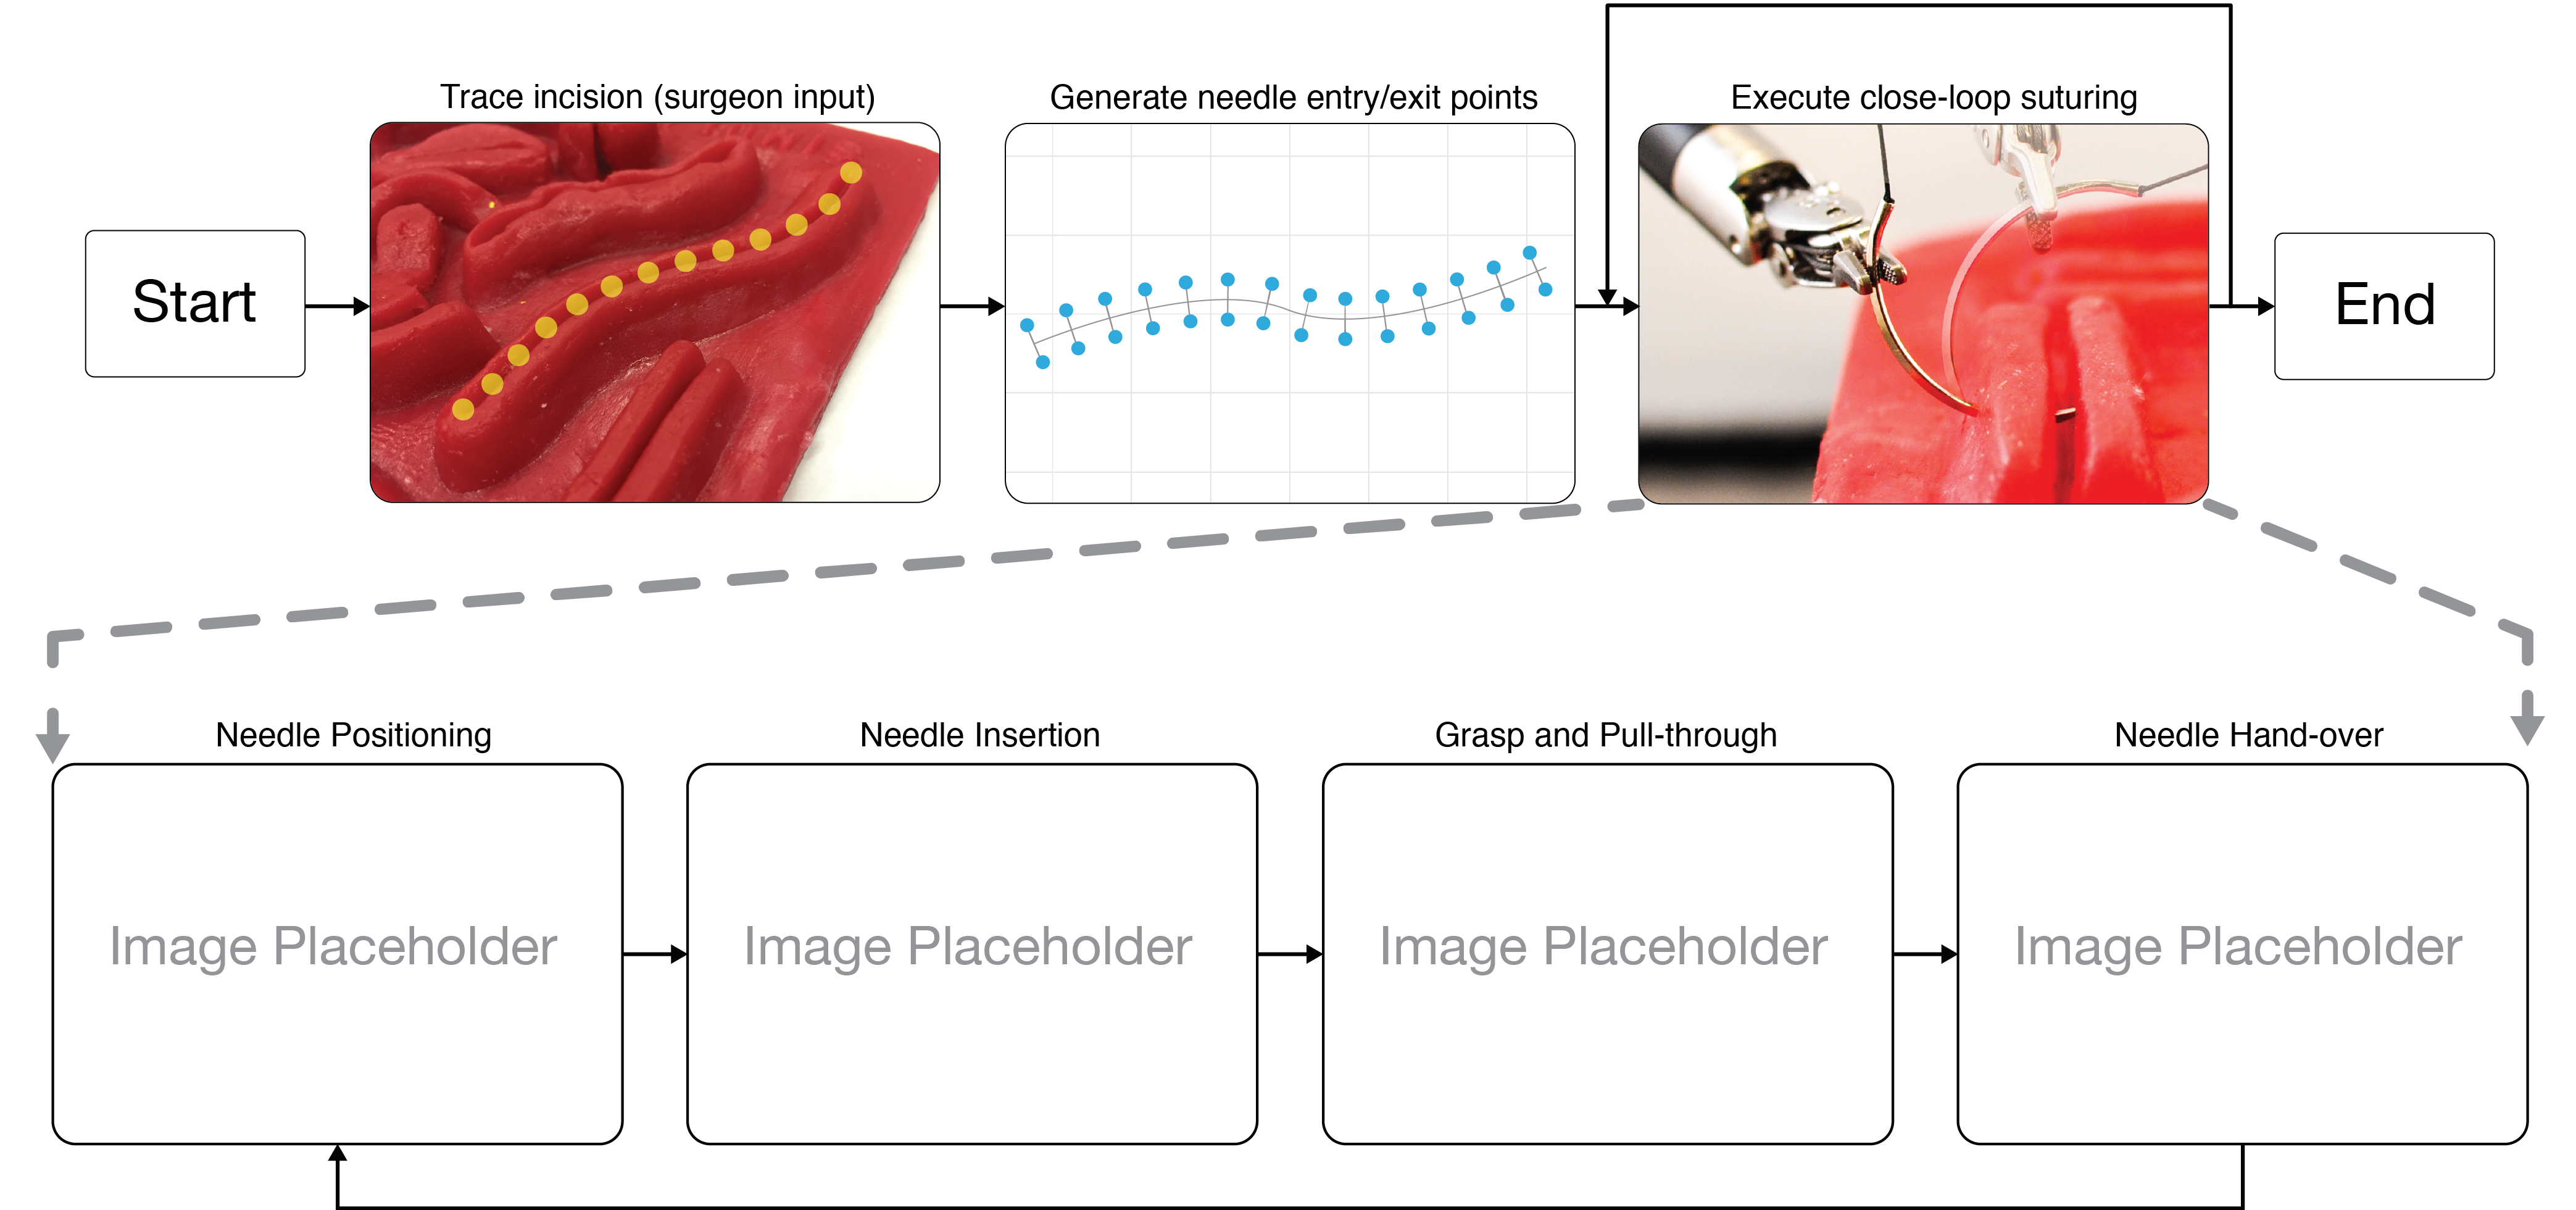
\includegraphics[width=0.9\linewidth]{figures/fsm}
% \vspace{-5pt}
\caption{\todo{Placeholder Figure} The Figure illustrate the algorithmic pipeline.The system receives a trace of the wound to suture along with wound width and depth. Step 2 calculates appropriate number of suture throws and entry/exit points. The suture throws are then repeated until success. Step 3  consists of 4 steps: Needle Positioning, Needle Insertion, Grasp and Pull Through and Needle Hand-off, in accordance with the Manual Labels in the JIGSAWS dataset. Needle Positioning and Needle Insertion is planned using Needle Path Planner, and Needle Grasp and Needle hand-off steps are performed under closed loop operation with needle tracking.}
\label{fig:fsm}
\vspace{-10pt}
\end{figure*}

%==START SECTION==============================
\section{Related Work}
\label{sec:relWork}
%============================================
% Robot assisted surgical systems have been used in a number of surgical interventions~\cite{alterovitz2008motion,Beasley2012,Taylor2008,Wolf2009}.
% Autonomous control of surgical robotic platforms may offer enhancements such as higher precision, higher speed, and lower tissue damage.

% As these authors summarize, contemporary RSA's primarily act as surgical extenders operated directly by the surgeon at all times and may extend human capabilities. Autonomous robotic systems beyond surgical extenders are largely at the experimental level.
% Although academic availability of RSAs such as \textit{Intuitive Surgical} dVRK~\cite{Kazanzides2014} and the Raven II~\cite{hannaford2013raven} system have accelerated recent developments. Task-level autonomy in repetitive and kinematically difficult tasks such as tissue dissection, and suturing may reduce fatigue and operative time. 




% \noindent \textbf{Related Work in Robotic Surgical Automation:}\\
Robot assisted surgical systems have been used in a number of surgical interventions~\cite{Taylor2008,alterovitz2008motion,Wolf2009,Beasley2012}.
Moustris et al.~\cite{Moustris2011} and Kranzfelder et al.~\cite{kranzfelder2013toward} have reviewed recent developments in semi-autonomous and autonomous execution of various surgical procedures. 
Further algorithms for active exploration in tumor localization~\cite{Nichols2013Autonomous}, and tumor ablation~\cite{Hu2015Semi} have also been explored. Our previous work~\cite{Kehoe2014Autonomous} used motion planning to perform multilateral surgical debridement using the Raven II surgical robot.

Surgical training in residents is evaluated using a basis set of  procedures~\cite{stegemann2013fundamental}, the \textit{Fundamental Skills of Robotic Surgery~(FSRS)}, that are representative of frequent sub-tasks experienced by most robot-assisted laparoscopic surgeons~\cite{Ritter2007,dulan2012developing, stegemann2013fundamental}. 
% As described Stegemann et al., the skills can be classified in four groups: (a) Basic Console operation, (b) Psychomotor Skills, (c) Basic Surgery Skills and (d) Intermediate Surgery Skills. ~\cite{stegemann2013fundamental}
It is often observed that procedures are composed of long sequences of subtasks, which are not directly amenable to automation.
Such multi-step procedures can be divided into simpler sub-tasks. 
Hence taking a step towards automation in the context of surgery, Hager et al. proposed a ``Language of Surgery" with ``surgemes" analogous to phonemes~\cite{Lin2006,Reiley2009,Varadarajan2009}.

This has led to a line of work in segmentation of demonstrations into meaningful motion sequences has been extensively studied~\cite{Konidaris2011,Niekum2015,Gienger2010, lea2015improved}. Manual segmentation of surgemes in demonstrations have been used for understanding and recognizing surgical skills and sub-tasks, and for evaluating surgeon skills~\cite{Reiley2009,Varadarajan2009}.
Our recent results on segmentation of task demonstrations~\cite{krishnan2015tsc} demonstrates that unsupervised recovery of semantic transitions is feasible and can be analyzed to construct Finite State Machines~(FSM) for these multi-step procedures.
\citet{Murali2015Learning} showed that finite state machines can be built with a learning by observation approach for robust automation in surgical subtasks involving cutting by provisioning for failure recovery behavior.

\vspace{3pt}
\noindent\textbf{Automation of Suturing: }
Suturing and knot tying have been explored on various occasions in recent past. Starting in early 2000s, \citet{Kang2000Autonomous} developed mathods that focused on the low level control necessary
to automate surgical subtasks such as suturing and knot tying.
Later on, \citet{Mayer2006System} used a recurrent neural net as part of a controller to learn knot tying motion primitives from human demonstrations.\citet{Berg2010Superhuman} used iterative learning control to extract smooth trajectories for performing knot tying at super human speeds. More recently, \citet{Schulman2013Case} used a learning by demonstration approach to warp recorded
expert demonstrations and performing suturing using a simulation of the Raven II. And \citet{Padoy2011} demonstrated execution of a human-robot collaborative suturing task on the DVRK platform. \todo{differentiate from padoy}

% \subsection{Related Work in Motion Planning in Medical Applications}
\vspace{3pt}
\noindent \textbf{Need for planning in suturing: }
One of the main consideration in suturing is minimizing trauma while approximation of the wound. And the choice of needle is very important in it. The needle is chosen based on the \textit{bite length}, the chord length of the needle and \textit{bite width}, conveying the curvature of needle. The objective while suturing is to create an \textit{eversion} in the wound (outward facing bulge) to assist in healing\tocite without applying excessive local force to prevent necrosis. Surgeon best practices require a needle to "bite" the tissue orthogonally during insertion. Additionally, the needle must inserted along a constant curvature arc defined by the shape of the needle in order to minimize trauma to the neighboring tissue \cite{Jackson2013Needle}. These motion constraints are difficult for even expert surgeons to satisfy \cite{Kang2000Autonomous}.

Thus, suturing success is highly dependent on dexterity in needle handling. Incorrect placement of the needle in the gripper may result in a bent needle, difficult penetration of the skin, or an undesirable angle of entry into the tissue. And beyond the correct grasp, the trajectory for a good suture requires complex handling and movement along the curvature of the needle.

\citet{Jackson2013Needle} used surgeon best practices as reference to plan needle paths for suturing, but experimented without uncertainty for a single throw of a given needle. Since the needle tip is moving along a curved path to accommodate the needle curvature, path planning should account for curvature constraints. Recent results in motion planning have shown that optimization based planning is both faster and solver more instances of problems compared to sampling based planners.
Of particular mention is TrajOpt~\cite{Schulman2014Motion} that uses sequential convex optimization to generate locally optimal trajectories.
\citet{Duan2014Planning} leveraged trajOpt to generate curved paths for steerable needle path planning without uncertainty in simulation.

However, as with any real system, there are unmodeled uncertainties in gripper-needle and needle-tissue interactions, which can result in needle to drift from a plan. Hence, tracking needle pose under uncertainty and trajectory plans to account for future uncertainty in control-action mapping can improve robustness. 
Recently, \cite{Kahn2015Active} used belief space optimization to actively explore unstructured environments in order to grasp occluded objects and \cite{Sun2014Motion} developed a motion planner that considers motion and sensor uncertainty while guiding steerable needles in a 3D anatomy.\todo{difference from sun2014motion}
Similarly, there have been explorations on needle tracking for surgical settings as showed by~\cite{wengert2007endoscopic, speidel2015image}.

\vspace{3pt}
\noindent \textbf{Why is our work novel? }
In this work, we use the \davinci Research Kit (dVRK) to perform an end to end continuous suture autonomously. We draw from state-of the art results in both manual labeling~\cite{gao2014jhu} and unsupervised learning of transitions~\cite{krishnan2015tsc}\todo{cite deep paper arxiv version}, to refine them into a robust FSM for the continuous running suturing task with multiple throws.

We segment each suturing throw into a sequence of four surgemes -- Needle Positioning, Needle Insertion, Needle Pull Through and Multilateral hand-off. We address the problem of choosing the correct needle size, positioning and insertion in a joint curvature constrained trajectory optimization problem. 
We use a Lie-Algebra re-parameterization of the pose to improve convergence of the gradient based method.
We also use needle tracking and re-planning to quantify and account for uncertainty using the belief state of the needle in the optimization. 
Use of belief over needle pose in place of deterministic pose, compensates for non-linear interactions with the tissue. Especially since the feedback is not perfect, our approach plans for a conservative path along with a “confidence” in completing the task.

\noindent \textbf{Gripper Augmentation for Needle Orientation: }
Experimental evaluation of the multilateral hand-off procedure needed multiple back and forth passes for achieveing the correct needle configuration in the insertion hand. The procedure still yielded frequent failures due to inaccurate goal poses of needle. To this end, we have devised a novel needle alignment mount for the gripper jaw that passively guides the needle into a known pose upon gripper closure. The device improves needle hand-off accuracy by \todo{x\%} compared to using current needle driver; and hence reduces the need for re-alignment before pushing needle in tissue.  

Automation can be highly beneficial in suturing with a reparametrization the complex motions necessary to effectively perform a stitch. Further, surgical automation can enable semi-supervised surgery by providing surgeons with an ability to input task level commands instead of direct low level control at all points in the surgery. This work is one of the first to present RMIS experiments with autonomous continuous suturing, made possible by a combination of optimization, needle tracking and custom automation enabling hardware.

% supervisory role and high level commands to direct the robot to desired suture locations.

%  Find a better constraint 

% Optimization-based motion planning applied to automating a surgical subtask
% Optimal needle size selection based on surgical environment
% Using lie algebra to optimize over the manifold
% Needle tracking that is robust to partial collusions
% Closed-loop automation of continuous surgical suturing
% Combine needle-tracking with motion planning
% Close-loop planning for optimal hand-off
% Generation of plans accounting for uncertainty



% Why BSP?
% BSP can allow one to account for sources of uncertainty associated with a surgical environment
% Tissue is highly deformable making predictions or simulations of its behavior very difficult.
% Visual feedback can be very noisy
% objects of interest are small (needles, tooltips)
% highly specular surfaces make it difficult to use RGBD sensors
% Modeling the uncertainty can allow the agent to quantify to compute a measure of “confidence” in completing the task (essential in a surgical environment):
% Type-I: Confidence at goal
% Type-II: chances of intermittent failure (drifts off the successful tube of trajectories)
% At each point have a running estimate of both of these measures and possibly create a composite “Confidence” score.


% We try to quantify and account for uncertainty in surgical domain. 
% We use trajectory optimization in belief space to compute curvature constrained, locally optimal trajectories using sequential convex programming. 
% We propose objective criteria to evaluating the quality of a needle trajectory
% We propose a method for selecting the right needle for a specific suturing task.
% We will demonstrate our work on dVRK.

\end{document}
